% Created 2013-02-04 Mon 14:15
\documentclass{article}
\usepackage[utf8]{inputenc}
\usepackage{fixltx2e}
\usepackage{url}
\usepackage{graphicx}
\usepackage{minted}
\usepackage{color}
\usepackage{longtable}
\usepackage{float}
\usepackage{wrapfig}
\usepackage{soul}
\usepackage{textcomp}
\usepackage{amsmath}
\usepackage{marvosym}
\usepackage{wasysym}
\usepackage{latexsym}
\usepackage{amssymb}
\usepackage[linktocpage,
  pdfstartview=FitH,
  colorlinks,
  linkcolor=blue,
  anchorcolor=blue,
  citecolor=blue,
  filecolor=blue,
  menucolor=blue,
  urlcolor=blue]{hyperref}
\usepackage{attachfile}
\tolerance=1000
\providecommand{\alert}[1]{\textbf{#1}}

\title{Homework 1 - Due 2/13/2013}
\author{John Kitchin}
\date{2013-02-04 Mon}
\hypersetup{
  pdfkeywords={},
  pdfsubject={},
  pdfcreator={Emacs Org-mode version 7.9.3a}}

\begin{document}

\maketitle

\setcounter{tocdepth}{3}
\tableofcontents
\vspace*{1cm}

\section{Compute the distance between the (111) planes of Ag.}
\label{sec-1}

Use the experimental lattice constant of Ag.
\subsection{solution \textbf{:solution:}}
\label{sec-1-1}

We use the reciprocal metric tensor to directly compute the spacings. It does not matter which unit cell you choose.

\begin{minted}[frame=lines,fontsize=\scriptsize,linenos]{python}
import numpy as np

a = 4.09

uc = np.array([[a, 0, 0],
               [0, a, 0],
               [0, 0, a]])

ucstar = np.linalg.inv(uc).T

gstar = np.dot(ucstar, ucstar.T)

v = [1, 1, 1]
d_111 = np.sqrt(np.dot(v, np.dot(gstar, v)))

print 'The spacing between the (111) planes is {0} angstroms.'.format(1.0 / d_111)

# if you use the primitive cell
b = a/2.0
uc = np.array([[b, b, 0],
               [b, 0, b],
               [0, b, b]])

ucstar = np.linalg.inv(uc).T

gstar = np.dot(ucstar, ucstar.T)

v = [1, 1, 1]
d_111 = np.sqrt(np.dot(v, np.dot(gstar, v)))

print 'The spacing between the (111) planes is {0} angstroms.'.format(1.0 / d_111)
\end{minted}

\begin{verbatim}
 The spacing between the (111) planes is 2.36136260099 angstroms.
 The spacing between the (111) planes is 2.36136260099 angstroms.
\end{verbatim}
\section{Angles and distances}
\label{sec-2}

Compute the length of the vector indicated by D, and the angle indicated by A. You can assume the unit cell is a cube with length of 3.6 nm on each side.

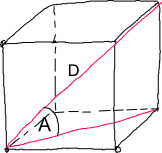
\includegraphics[width=.9\linewidth]{./images/hwk1-cube.png}
\subsection{solution \textbf{:solution:}}
\label{sec-2-1}

The most general approach is to define the unit cell, and then define the vector in the unit cell coordinate system, and compute the distance.


\begin{minted}[frame=lines,fontsize=\scriptsize,linenos]{python}
import numpy as np

a= 3.6
uc = np.array([[a, 0, 0],
               [0, a, 0],
               [0, 0, a]])

g = np.dot(uc, uc.T)

P = [1, 1, 1]

d = np.sqrt(np.dot(np.dot(P, g), P))
print d
\end{minted}

\begin{verbatim}
 6.23538290725
\end{verbatim}

For the angle, 


\begin{minted}[frame=lines,fontsize=\scriptsize,linenos]{python}
import numpy as np

a= 3.6
uc = np.array([[a, 0, 0],
               [0, a, 0],
               [0, 0, a]])

g = np.dot(uc, uc.T)

P = [1, 1, 0]
Q = [1, 1, 1]

lp = np.sqrt(np.dot(P, np.dot(g, P)))
lq = np.sqrt(np.dot(Q, np.dot(g, Q)))

print lp, lq

theta = np.arccos(np.dot(P, np.dot(g, Q))/(lp * lq))
print theta * 180.0 / np.pi
\end{minted}

\begin{verbatim}
 5.09116882454 6.23538290725
 35.2643896828
 54.7356103172
\end{verbatim}
\section{Coordinate system transformations}
\label{sec-3}


The unit cell of a material is given by:

\begin{verbatim}
     4.2266540199664249    0.0000000000000000    0.0000000000000000
     0.0000000000000000    4.2266540199664249    0.0000000000000000
     0.0000000000000000    0.0000000000000000    2.6888359272289208
\end{verbatim}

The coordinates of the atoms in the unit cell are given in fractional coordinates as:

\begin{verbatim}
  0.0000000000000000  0.0000000000000000  0.0000000000000000
  0.5000000000000000  0.5000000000000000  0.5000000000000000
  0.3067891334429594  0.3067891334429594  0.0000000000000000
  0.6932108665570406  0.6932108665570406  0.0000000000000000
  0.1932108665570406  0.8067891334429594  0.5000000000000000
  0.8067891334429594  0.1932108665570406  0.5000000000000000
\end{verbatim}

Compute the Cartesian coordinates of each atom.
\subsection{Solution \textbf{:solution:}}
\label{sec-3-1}


We simply have to compute for each position (s1, s2, s3) the vector sum of s1*A + s2*B + s3*C where A, B, C are the unit cell vectors. We have a matrix where row 1 is A, row 2 is B, and row 3 is C.

Let this be our matrix:

\[M = \begin{array}{ccc} a1 & a2 & a3 \\
                       b1 & b2 & b3 \\
                       c1 & c2 & c3 \end{array} \]

We end up with the following equations:

p$_x$ = s1*a1 + s2*b1 + s3*c1
p$_y$ = s1*a2 + s2*b2 + s3*c2
p$_z$ = s1*a3 + s2*b3 + s3*c3

or in matrix form:

\[ [\begin{array}{ccc}s1 & s2 & s3\end{array}] %
               \cdot \left[\begin{array}{ccc} a1 & a2 & a3 \\
               b1 & b2 & b3 \\
               c1 & c2 & c3 \end{array} \right] = [ \begin{array}{ccc} p_x & p_y & p_z\end{array}] \]
   


\begin{minted}[frame=lines,fontsize=\scriptsize,linenos]{python}
import numpy as np

uc = np.array([[4.2266540199664249,    0.0000000000000000,    0.0000000000000000],
               [0.0000000000000000,    4.2266540199664249,    0.0000000000000000],
               [0.0000000000000000,    0.0000000000000000,    2.6888359272289208]])


sp = np.array([[  0.0000000000000000,  0.0000000000000000,  0.0000000000000000],
               [  0.5000000000000000,  0.5000000000000000,  0.5000000000000000],
               [  0.3067891334429594,  0.3067891334429594,  0.0000000000000000],
               [  0.6932108665570406,  0.6932108665570406,  0.0000000000000000],
               [  0.1932108665570406,  0.8067891334429594,  0.5000000000000000],
               [  0.8067891334429594,  0.1932108665570406,  0.5000000000000000]])

cp = np.dot(sp, uc)

print cp



print 'Alternative approach'
# alternate approach
for row in sp:
    print uc[0]*row[0] + uc[1]*row[1] + uc[2]*row[2]
#print uc[0] * sp[:,0] + uc[1] * sp[:,1] + uc[2] * sp[:,2]
\end{minted}


\begin{verbatim}
[[ 0.          0.          0.        ]
 [ 2.11332701  2.11332701  1.34441796]
 [ 1.29669152  1.29669152  0.        ]
 [ 2.9299625   2.9299625   0.        ]
 [ 0.81663549  3.41001853  1.34441796]
 [ 3.41001853  0.81663549  1.34441796]]
Alternative approach
[ 0.  0.  0.]
[ 2.11332701  2.11332701  1.34441796]
[ 1.29669152  1.29669152  0.        ]
[ 2.9299625  2.9299625  0.       ]
[ 0.81663549  3.41001853  1.34441796]
[ 3.41001853  0.81663549  1.34441796]
\end{verbatim}
\section{Computing unit cell parameters}
\label{sec-4}

For the following unit cell (in rows), compute the length of each vector, and the angle between the vectors, e.g. the ``a b c $\alpha$ $\beta$ $\gamma$'' representation. 


\begin{verbatim}
3.817   -0.011  -0.243
-0.011  3.817   -0.243
-1.519  -1.519  4.986
\end{verbatim}
\subsection{solution \textbf{:solution:}}
\label{sec-4-1}


\begin{minted}[frame=lines,fontsize=\scriptsize,linenos]{python}
import numpy as np
from Scientific.Geometry import Vector
A = Vector([3.817,      -0.011, -0.243])
B = Vector([-0.011,     3.817,  -0.243])
C = Vector([-1.519,     -1.519, 4.986])

a = A.length()
b = B.length()
c = C.length()
alpha = B.angle(C) * 180.0 / np.pi
beta = A.angle(C) * 180.0 / np.pi
gamma = A.angle(B) * 180.0 / np.pi

print 'a={a:1.2f} b={b:1.2f} c={c:1.2f} alpha={alpha:1.2f} deg beta={beta:1.2f} deg gamma={gamma:1.2f} deg'.format(**locals())
\end{minted}

\begin{verbatim}
 a=3.82 b=3.82 c=5.43 alpha=109.68 deg beta=109.68 deg gamma=90.10 deg
\end{verbatim}
\section{Computing fractional coordinates}
\label{sec-5}

Given this unit cell (in rows)

\begin{verbatim}
3.817   -0.011  -0.243
-0.011  3.817   -0.243
-1.519  -1.519  4.986
\end{verbatim}

And atoms at these cartesian coordinates:


\begin{verbatim}
 [[ 1.23141,   0.239958,  3.102345]
  [ 1.05559,   2.047042,  1.397655]
  [-0.626458,  2.21009,   3.890655]
  [ 2.913458,  0.07691,   0.609345]
  [ 1.004314,  0.139186,  1.125   ]
  [ 1.282686,  2.147814,  3.375   ]]
\end{verbatim}

Compute the fractional coordinates of each atom in the unit cell.
\subsection{solution \textbf{:solution:}}
\label{sec-5-1}


\begin{minted}[frame=lines,fontsize=\scriptsize,linenos]{python}
import numpy as np

uc = np.array([[3.817,  -0.011, -0.243],
               [-0.011, 3.817,  -0.243],
               [-1.519, -1.519, 4.986]])

cp = np.array([[ 1.23141,   0.239958,  3.102345],
                 [ 1.05559,   2.047042,  1.397655],
                 [-0.626458,  2.21009,   3.890655],
                 [ 2.913458,  0.07691,   0.609345],
                 [ 1.004314,  0.139186,  1.125   ],
                 [ 1.282686,  2.147814,  3.375   ]])

print np.dot(np.linalg.inv(uc.T), cp.T).T

print 'alternative, and equivalent linear algebra'
print np.dot(cp, np.linalg.inv(uc))
\end{minted}


\begin{verbatim}
[[ 0.589  0.33   0.667]
 [ 0.411  0.67   0.333]
 [ 0.17   0.911  0.833]
 [ 0.83   0.089  0.167]
 [ 0.363  0.137  0.25 ]
 [ 0.637  0.863  0.75 ]]
alternative, and equivalent linear algebra
[[ 0.589  0.33   0.667]
 [ 0.411  0.67   0.333]
 [ 0.17   0.911  0.833]
 [ 0.83   0.089  0.167]
 [ 0.363  0.137  0.25 ]
 [ 0.637  0.863  0.75 ]]
\end{verbatim}

\end{document}
